\documentclass{article}
\usepackage[utf8]{inputenc}
\usepackage[T1]{fontenc}
\usepackage{graphicx}
\usepackage{hyperref}
\usepackage{geometry}
\geometry{margin=1in}

\title{THISTLE}
\date{Encyclopaedia Britannica (1771)}

\begin{document}
\maketitle

\section*{Historical source}
\textbf{Entry ID:} \texttt{entry-thistle-1614} \\
\textbf{Volume ID:} 144133903 \\
\textbf{Character Count:} 2021

\subsection*{Extracted Text}
THISTLE, in botany. See Carousus.

\_Order of Life\_ THISTES, or of BX Anakaw, a military order of neighborhood in Scotland, the rife and infiltration whereof is variously related by different authors. Leley, bilbp of Roofs, reports, that the girls below the battle between Chichling king of Northumberland, and Humpes king of the Pilots, a bright crois, in form of that whercen on St Andrew (the under false is Scotland) fafferent majority appears to the Hunges; who being grand the victory, ever after bore the figure of that crois on his baners. Others affer, that Auchana King of Scotland ifn influenced the orders, after having any of the famous league offensive and defensive with Charlemagae king of France. But although he still had been acknowledged as the Jhnol of the kingdom of Sozbank from the reign of Achaiu, yet fome refer the beginning of this order to Charles VII, of France. Others place the foundation of as far as the year z too.

The chief and principal edge is a gold collar compo- feel fullfills and griping of me indicated with amules of golf, having freedom thereto the image of St Andrew with his crois, and the motto, NMO THE IMPUNE LA CITY.

The ordinary or common origin worn by the knights, is a flat of four River points, and over them a green circled, borders and offered through pink, containing the find motto, and in the camera is a thilfe proper, all which is embroidered on their left breastf, and womb with the collay, with a great method over the shoulder, and brought under the right arm i pender thereto is the iimage of St Andrew, with his crois, in a purple robe, within an oral of gold canamelled very, with the former motto - but femonettes they were, existed in the June manner, a hittle crowned.

Also, the time of the reformation, this order was dropped, till James II: of England refumed it, by creating eight knights I however, the resolution unifedit is again, and are why neglected the mena Anne, no 2023, reduced to the primitive delges of twelve knights of St Andrews.



\section*{Source record}
\begin{itemize}
\item \textbf{Dataset:} \texttt{NationalLibraryOfScotland/encyclopaedia\_britannica\_illustrated}
\item \textbf{Dataset Revision:} \texttt{309f765b1ecc83e0a7f7762e44b4a927a7555443}
\item \textbf{Page ID:} \texttt{britannica:309f765b1ecc83e0a7f7762e44b4a927a7555443:train:1614} \\
  \textbf{Filename:} \texttt{page-1614-ea352b487d65.jpg} \\
  \textbf{Row Index:} 1614 \\
  \textbf{SHA256:} \texttt{ea352b487d650c71...}
\end{itemize}

\begin{figure}[h]
\centering
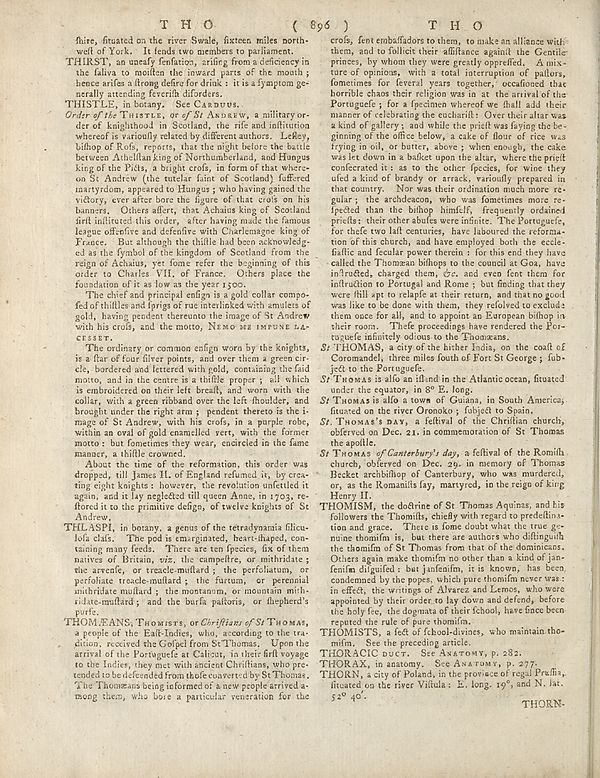
\includegraphics[width=0.85\textwidth]{../scans/page-1614-ea352b487d65.jpg}
\caption*{Source scan: \texttt{page-1614-ea352b487d65.jpg}}
\end{figure}

\end{document}
